\chapter{性能分析}

在完成\ref{chap3}中描述性能的性能优化后,将其部署在测试平台下,测试平台由 3 台计算机构成,硬件配置如下所示:

1. 操作系统: Ubuntu 16.04.2 LTS (GNU/Linux 4.4.0-72-generic x86\_64)

2. 中央处理器: Intel(R) Xeon(R) CPU E5-2620 v2 @ 2.10GHz

3. 内存:63149 MB

4. 网卡:Ethernet controller: Broadcom Corporation NetXtreme II BCM57800 1/10 Gigabit Ethernet * 4

5. 硬盘:1.75 TB 机械硬盘

相比\ref{chap3}中的硬件环境,差别体现在计算机之间的物理距离更近,计算机之间的网络延迟更低,使用 ping 命令进行测试得出网络节点间的网络延迟从平均 2.295 ms 降低到了平均 0.496 ms,更利于分布式平台的搭建。
M. Joseph 与 P. Pandya 等人指出在实时系统中主要存在两方面的性能问题,一方面是每个请求的平均响应时间与最差响应时间,另一方面是系统在不丢失任何请求的情况下可以处理的请求数量\upcite{joseph1986finding}。本章主要从请求响应时间与响应请求数量两方面进行分析。

\section{请求响应时间分析}
Grigorik 等人通过分析大量用户数据,指出用户即使平时生活中接触不到毫秒级别的时间,但是仍能明显感受到毫秒级别的延迟。延迟在 100ms 以内的时候,用户会认为立即得到了响应;在 100 \~ 300 ms 之间,用户会感觉到轻微的延迟;300 \~ 1000 ms 之间,用户仅仅认为系统工作正常,但体验较差;当延迟达到 1000 ms 之上的时候,用户会去做其他工作,不时查看任务是否已经完成;如果延迟达到了 10,000ms 的时候,用户开始怀疑任务程序是否出现了问题,放弃执行任务\upcite{grigorik2013high}。因此,为了满足神经科学家流畅地进行对神经元的实时编辑任务,需要使服务器响应时间控制在 100ms 以内。需要注意的是,用户真正感受到的响应时间还包括前端可视化工作所需的计算时间以及浏览器的渲染时间等,这对服务器的响应时间有了更高的要求。

由于网络服务器与客户端之间的通讯建立在 TCP 协议之上,而 TCP 协议广泛采用慢启动作为网络流量控制算法,网络延迟对于小文件的传输影响巨大。在不考虑服务器对数据的处理时间的情况下,对于传输一个 64KB 的神经元结构,分布式网络节点间的理论响应时间可由下式计算:
$$Time=RTT*\lceil log_2(\frac{N}{initial~cwnd}) \rceil$$
式中 $RTT$ 代表发送方与接收方之间的往返所需的时间,对应到\ref{chap3}描述的原始平台为 2.295 ms,在本章中搭建的测试平台为 0.496 ms。$initial~cwnd$ 代表初始拥塞控制窗口大小,根据 RFC 6928 中的规定,原始平台与测试平台均采用了 1,460 bytes 作为初始拥塞窗口大小\upcite{chu2013increasing}。将上述数据带入公式中计算可知,原始平台需要 6.885 ms,本章描述的平台只需 1.488 ms,响应时间降低了 78.39\%,性能提升显著。

测试主要针对获如下三类调用量较大的 API 进行测试:

1. 用户原始图像列表相关 API。

2. 用户对神经元结构进行操作的相关 API。

3. 结构脑胞体相关 API。

在这部分的测试中,模拟 1,000 名用户进行编辑,每名用户的编辑动作进行 3 种操作各 100 个,所有用户共计进行 300,000 次 API 调用。测试结果如图 \ref{response} 所示,响应时间的分布如图 \ref{responsedis} 所示。从图中可以明显的看出绝大多数请求的响应时间集中在 0-20 ms 之间,极少数请求的响应时间超过了 100 ms。按照 Grigorik 分析大量用户数据得出的标准,满足了实时操作的要求。

\begin{figure}[!ht]
\centering
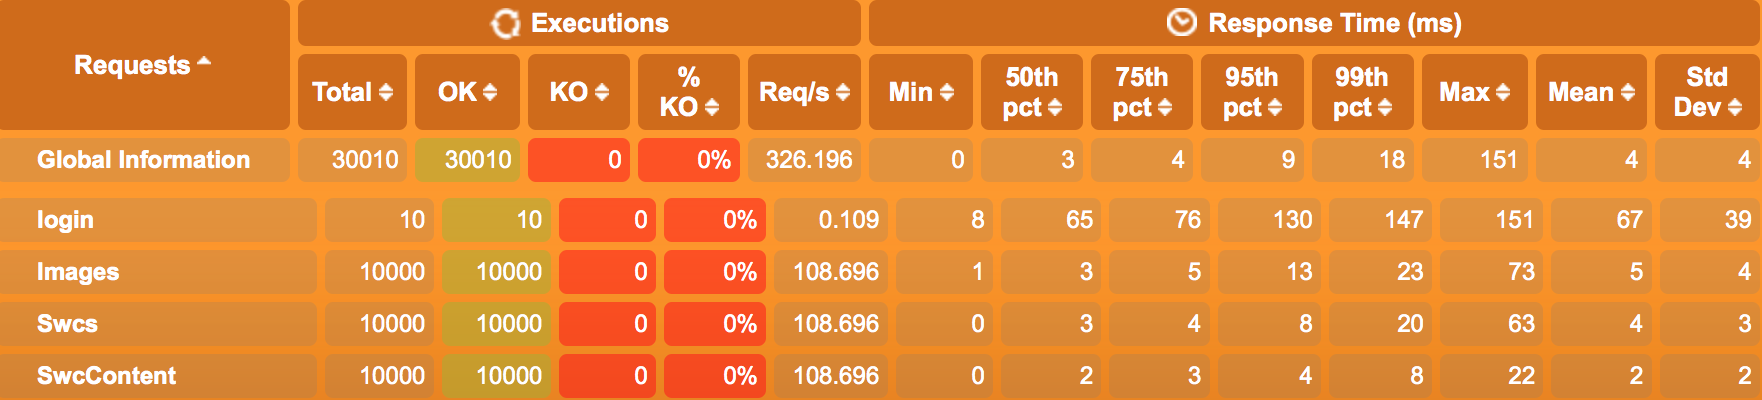
\includegraphics[width=148mm]{images/response}
\caption{请求响应时间,图中 Login 代表用户登录的请求,Images 代表获取用户原始图像列表相关 API 的响应时间,Swcs 代表用户对神经元结构进行操作的相关 API 的响应时间,SwcContent 代表用户获取结构脑胞体的响应时间。}
\label{response}
\end{figure}

\begin{figure}[!ht]
\centering
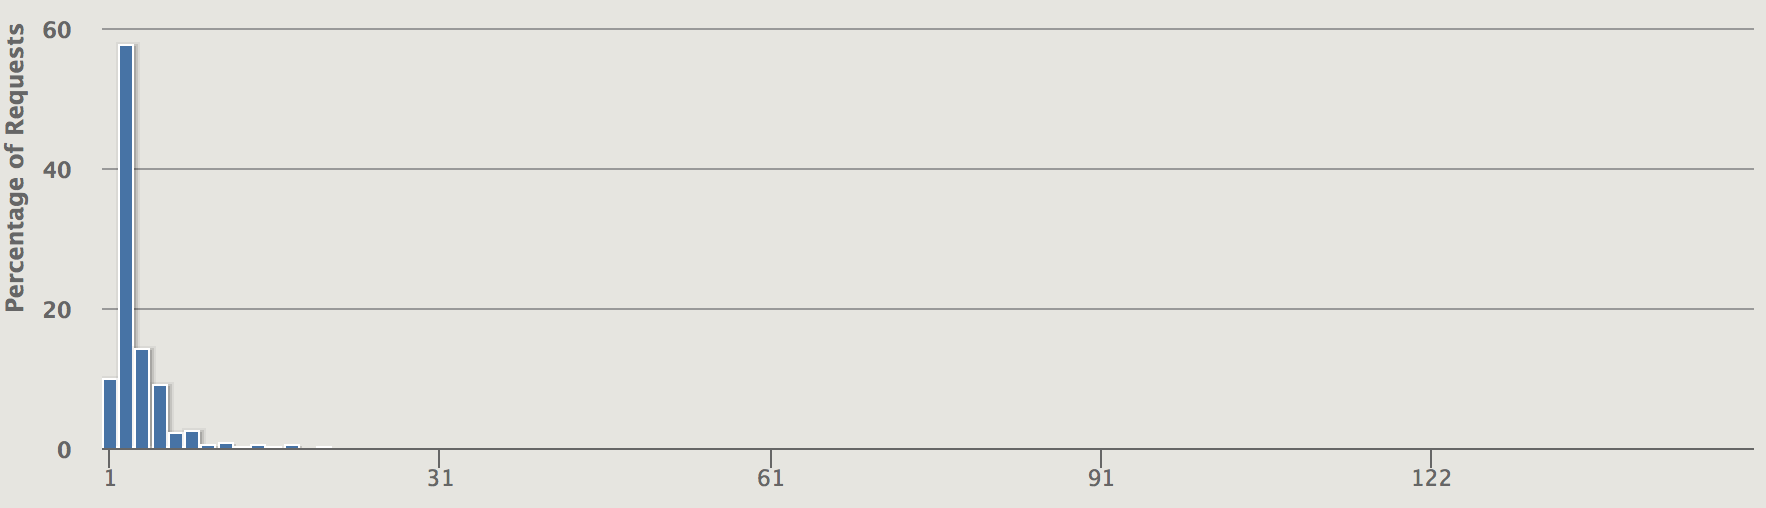
\includegraphics[width=148mm]{images/responsedis}
\caption{所有请求响应时间的分布,可以明显地看出绝大多数请求的响应时间集中在 0-20 ms 之间,极少数请求的响应时间超过了 100 ms。}
\label{responsedis}
\end{figure}

\begin{figure}[!ht]
\centering
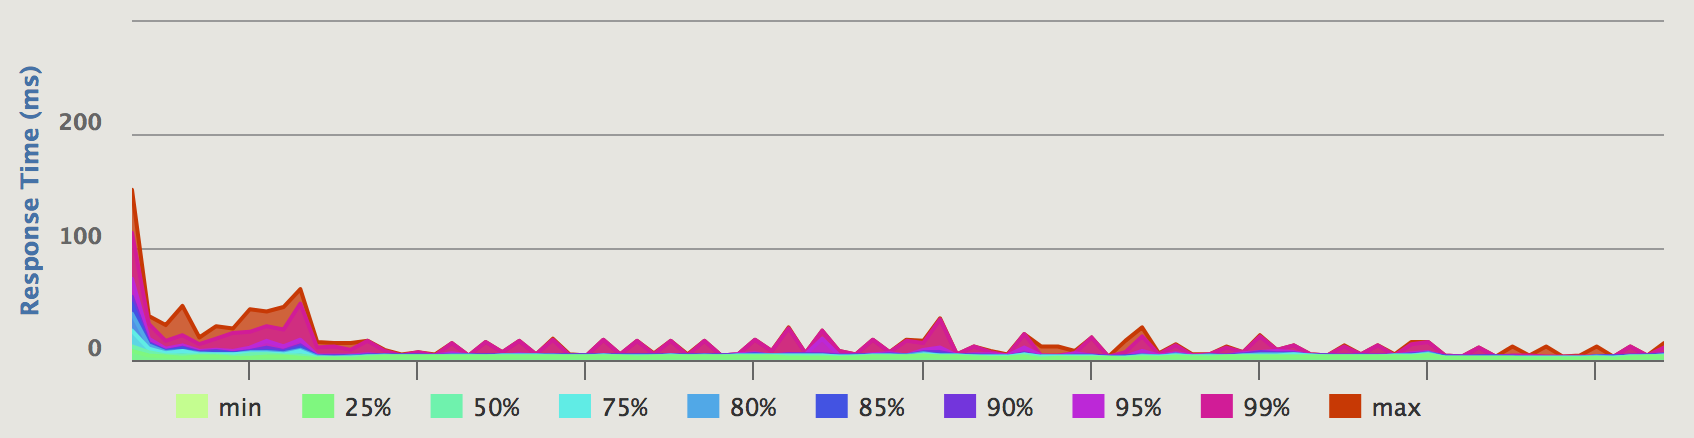
\includegraphics[width=148mm]{images/responsetime}
\caption{请求响应时间随时间的变化,不同颜色标明了不同比例请求所使用的时间。测试开始时,由于没有缓存,请求的响应时间较高,随着时间的推移,绝大多数的请求被服务器端或者浏览器端缓存下来,响应时间趋于平缓。}
\label{responsetime}
\end{figure}

进一步分析响应时间随时间的变化,如图 \ref{responsetime} 所示,可以看出在测试开始时,由于没有缓存,请求的响应时间较高,随着时间的推移,绝大多数的请求被服务器端或者浏览器端缓存下来,响应时间趋于平缓。这说明了使用 Redis 与浏览器端缓存对性能的提升明显,将需要花费一百毫秒才能完成的计算任务降低到可以在毫秒级别内响应,另一方面也降低了服务器的计算压力,使得用户的体验更加流畅。

\begin{figure}[!ht]
\centering
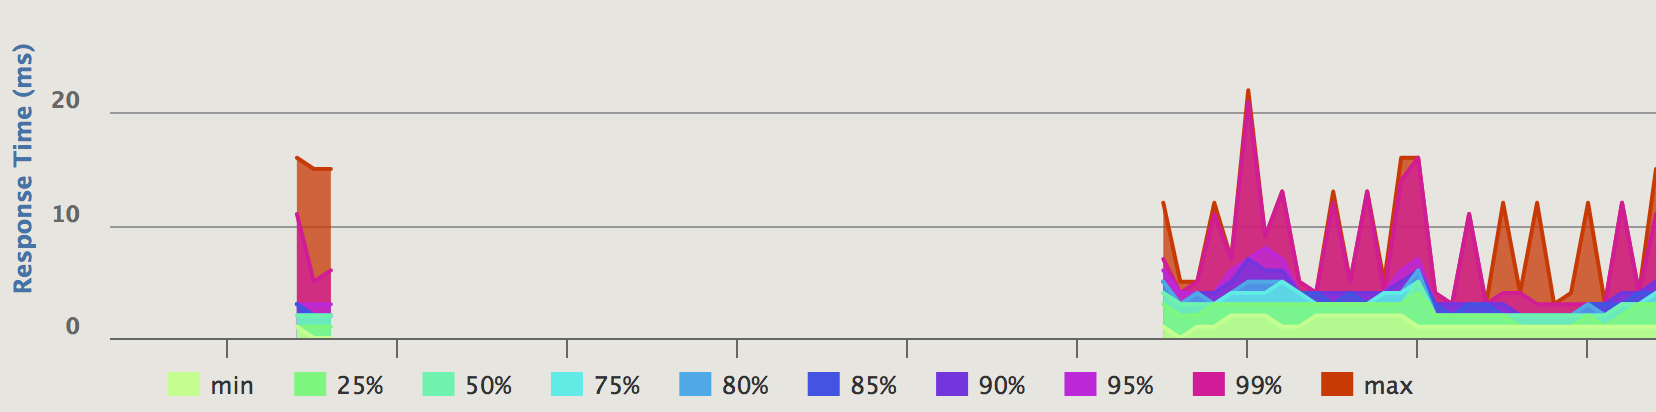
\includegraphics[width=148mm]{images/operation-res}
\caption{用户对神经元结构进行操作的相关 API 的响应时间的变化趋势}
\label{operation-res}
\end{figure}

\begin{figure}[!ht]
\centering
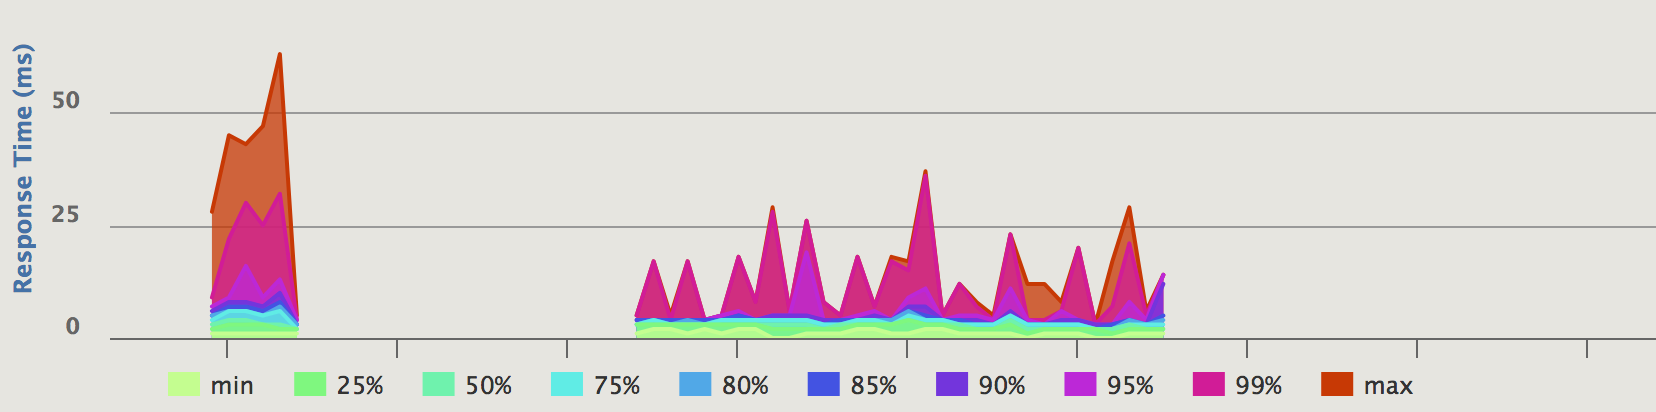
\includegraphics[width=148mm]{images/swc-c-res}
\caption{用户获取结构脑胞体的 API 的响应时间的变化趋势}
\label{swc-c-res}
\end{figure}

\begin{figure}[!ht]
\centering
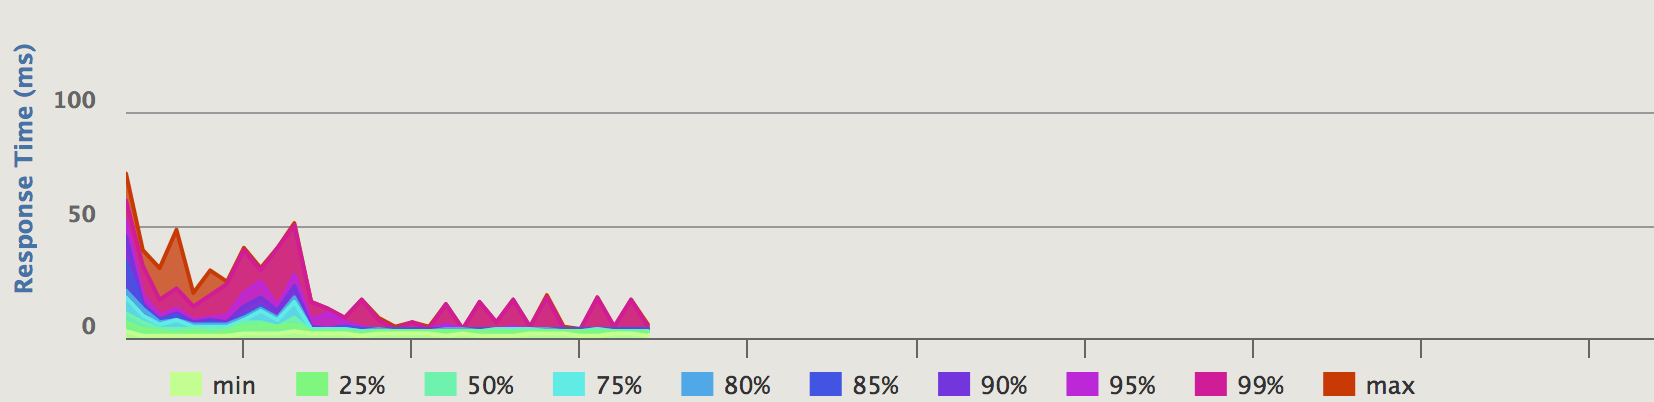
\includegraphics[width=148mm]{images/image-res}
\caption{获取用户原始图像信息的相关 API 的响应时间随时间的变化趋势}
\label{image-res}
\end{figure}

图 \ref{operation-res},\ref{swc-c-res} 与 \ref{image-res} 具体描述了三种 API 随时间变化的趋势。结合三幅图片可以明显地看出在不同时间段内模拟用户调用的 API 不同,模拟用户首先大量调用原始图像信息的相关 API,接着调用获取结构脑胞体的相关 API,最终调用编辑结构脑胞体的相关 API。另外一点重要的信息是,由于用户调用图像信息和结构脑胞体信息时经常重复,因此使用缓存的优化手段对性能影响明显,而用户操作往往不同,无法进行缓存。这一点反应在图片中是,在图 \ref{image-res} 与 \ref{swc-c-res} 中开始时响应时间较高,加入到缓存中后响应时间大幅降低,而图 \ref{operation-res} 响应时间一直维持在同一水平上,没有降低的趋势。

\section{响应请求数量分析}
为了支持多用户同时编辑,平台需要支持多用户同时在线,能够处理大量的并发请求。测试结果如图 \ref{requests} 所示。由于共有 1,000 名模拟用户,理论上并发请求最多可以达到 1,000。可以看到峰值最高接近 1,000 左右,没有出现因为请求过多超过服务器负载的情况。

\begin{figure}[!ht]
\centering
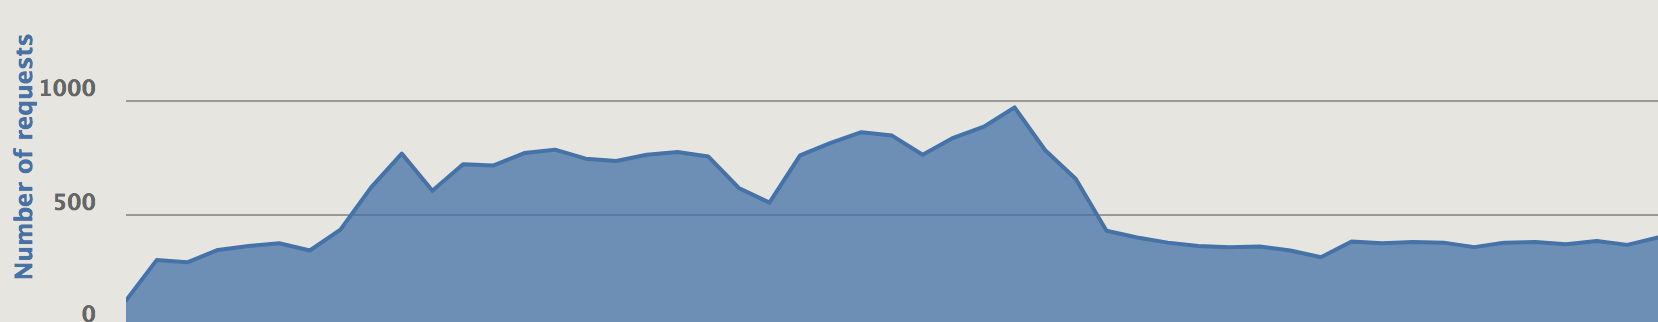
\includegraphics[width=148mm]{images/num-res}
\caption{每秒钟响应请求数量}
\label{requests}
\end{figure}

\section{本章小结}
本章详细描述了部署在测试平台的系统性能。通过详细的性能测试报告,说明了系统在平均情况下可以在数毫秒内做出响应,最差情况下也足以在两百毫秒内做出响应,满足了实时编辑的需求。同时,系统每秒钟可以至少处理一千次请求,足以支撑至少一千名用户同时在线编辑神经元结构,满足了团队协同工作的需求。




